\section{Robustness}\label{sec:robustness}

The checks here stand beside the confirmation map and outside the registered reading. Most ran
on the \NumSeedsDev{} development seeds and stand beside the development map on those seeds: the side checks,
the two bounds, the update scheme, the adoption rule with the network and the launch, and the chains of failure.
The exploratory side checks ran after the confirmation was read, on seeds kept for that purpose, and the size
check on its own seeds. Each subsection names its seeds.

\subsection{Side checks and bounds}

Eleven side checks rerun three launch levels (5\%, 20\% and 60\%, at an outside rate of 4.4\%), each with no
distress and at 2 points, six cells in all, on the development seeds with one setting changed. They are read beside the development map
on the same seeds. Halving or doubling the noise in the leaving rule, the low and the
high fixed cost, and pricing failures past the monthly fee cap at zero leave CPM's gains within a few per cent of
the development map's. Allowing five failure fees a month, not two, raises them. Cutting card lines in the
distress year raises failed payments in every arrangement and leaves CPM's gain unchanged. The record rule of
Section~\ref{sec:record}, here on the development seeds and three launch levels, gives the same picture: the pool serves
fewer bridges, and CPM's gains over both alternatives shrink but stay positive in every cell, with and without
distress (Table~\ref{tab:side}).

\begin{table}[htbp]\centering\small
\resizebox{\linewidth}{!}{% Written by scripts/paper_numbers.py from confirmation_quote.
\begin{tabular}{lrrrrrrrrr}
\toprule
 & \multicolumn{3}{c}{Gain over banks and cards} & \multicolumn{3}{c}{Gain over best-case DeFi} & \multicolumn{3}{c}{Bridges served at 2 points} \\
Launch participation & 5\% & 20\% & 60\% & 5\% & 20\% & 60\% & 5\% & 20\% & 60\% \\
\midrule
development map & \$119 & \$243 & \$465 & \$62 & \$124 & \$226 & 0.92 & 0.78 & 0.50 \\
\midrule
leaving noise halved & \$119 & \$244 & \$467 & \$61 & \$124 & \$227 & 0.93 & 0.81 & 0.52 \\
leaving noise doubled & \$119 & \$243 & \$460 & \$62 & \$125 & \$222 & 0.91 & 0.76 & 0.46 \\
fixed cost low & \$119 & \$244 & \$465 & \$62 & \$124 & \$226 & 0.92 & 0.77 & 0.47 \\
fixed cost high & \$119 & \$245 & \$465 & \$62 & \$125 & \$226 & 0.92 & 0.80 & 0.50 \\
entrants read the track record & \$116 & \$217 & \$396 & \$59 & \$98 & \$157 & 0.66 & 0.26 & 0.34 \\
entrants read it with noise & \$119 & \$236 & \$399 & \$61 & \$116 & \$160 & 0.81 & 0.47 & 0.32 \\
failures past the fee cap at zero & \$119 & \$244 & \$465 & \$62 & \$124 & \$226 & 0.92 & 0.78 & 0.50 \\
five failure fees a month & \$131 & \$265 & \$502 & \$76 & \$149 & \$268 & 0.89 & 0.74 & 0.46 \\
card lines cut in the distress year & \$119 & \$243 & \$465 & \$62 & \$124 & \$226 & 0.91 & 0.76 & 0.50 \\
half re-choose their buffer each month & \$118 & \$243 & \$459 & \$61 & \$124 & \$221 & 0.92 & 0.81 & 0.48 \\
15.3\% re-choose their buffer each month & \$117 & \$240 & \$449 & \$60 & \$120 & \$210 & 0.92 & 0.82 & 0.52 \\
\bottomrule
\end{tabular}
}
\caption{Side checks on three cells at an outside rate of 4.4\%, one setting changed in each, on the development
seeds: CPM's gain in money, in dollars a person a year with no distress, and bridges served in years 4 and 5 at 2
points of distress.}
\label{tab:side}
\end{table}

Two bounds rerun the whole development map on its seeds (Table~\ref{tab:bounds}). In the first the pool loses, and
prices, the published charge-off rate of each class of loan, where the model as built collects a written-off debt
later. The bridge price rises, as it must. CPM's gains are almost unchanged and every gain stays positive in every
cell. As many cells with no distress are stable (Persistent and passing the group clause on a majority of seeds,
the second view of Section~\ref{sec:measurement}) as on the development map. Fewer are stable under the
cash-advance bound as well, the table's last column.

The second is the outer bound on money paid to outside lenders. As built, the interest and fees households
pay to outside lenders and card issuers leave the household economy, so what a household saves by borrowing from
the pool counts as its gain. In the bound all that money returns to households in proportion to their
spending, as if they owned the lenders outright and lending cost nothing to supply. CPM's gain in money over
banks and cards falls by more than half but stays positive in every cell. Its gain in money over best-case DeFi
falls to zero. Its gain with completed purchases counted stays positive against both in every cell, and it fails
fewer payments than both in every cell. On a majority of seeds no cell is stable under this bound, because the
group clause is read in money against banks and cards.

The bound is exact about what the two kinds of gain are. Against best-case DeFi, CPM's gain in money is a
transfer: interest and fees households no longer pay to outside lenders. Its real gain is the payments that
no longer fail, delivered with the same real resources (Table~\ref{tab:gains}). How much of the transfer counts
as a gain to households depends on who owns the lenders. As built nobody in the model does, which leans toward
CPM; in the bound everybody does, which leans against it; households in fact own a small share. At the sourced
share, a tenth of lenders' income returning to households as the lenders' owners, the median gain in money is
\GainBanksShared{} over banks and cards and \GainDefiShared{} over best-case DeFi, read from the confirmation map as built with
no change in behaviour. On that reading the gain over best-case DeFi reaches zero only when a share of
\LenderShareZeroDefi{} of lenders' income returns to households.

\begin{table}[htbp]\centering\small
\resizebox{\linewidth}{!}{% Written by scripts/paper_numbers.py from confirmation_quote.
\begin{tabular}{lrrrrrrrrr}
\toprule
Map & Gain over banks & Gain over DeFi & Banks, purchases counted & DeFi, purchases counted & Every gain positive & Fewer failed payments & Bridge price & Stable as built & Stable both ways \\
\midrule
development map & \$296 & \$156 & \$611 & \$503 & 105 of 105 & 104 of 105 & 2.1\% & 14 of 21 & 11 of 21 \\
\midrule
loan losses at published rates & \$291 & \$151 & \$659 & \$499 & 105 of 105 & 105 of 105 & 5.5\% & 14 of 21 & 8 of 21 \\
lenders' interest returned & \$131 & $-$\$1.0 & \$413 & \$262 & 0 of 105 & 105 of 105 & 2.1\% & 0 of 21 & 0 of 21 \\
\bottomrule
\end{tabular}
}
\caption{The two bound maps beside the development map, each the whole grid on the same development seeds. Gains are medians over the
cells with no distress, in dollars a person a year, in money alone and with completed purchases at their price.
Counts of cells with every gain positive and with fewer failed payments are over the whole grid; the last two
columns count cells with no distress that are stable on a majority of seeds.}
\label{tab:bounds}
\end{table}

\subsection{The stress boundary in finer steps}

The grid's distress levels are half a point apart. On the \NumSeedsDev{} development seeds a finer cut between 1.5 and 2
points at three launch levels shows the shape of the boundary (Table~\ref{tab:boundary}). Bridges served fall
smoothly with distress at every launch level, with no cliff. On a majority of these seeds owners run on the
pool from \BoundaryFortyFive{} at a launch of 45\%, and at launches of 20\% and 30\% at no level up to 2 points.
On the \NumSeeds{} confirmation seeds runs are more frequent (Table~\ref{tab:stress}); the cut shows how bridges served
fall, not where the boundary lies. The nine runs of this cut with no distress repeat cells of the development map
and reproduce all \BoundaryRepeatValues{} of their stored values.

\begin{table}[htbp]\centering\small
\resizebox{\linewidth}{!}{% Written by scripts/paper_numbers.py from confirmation_quote.
\begin{tabular}{rrrrrrr}
\toprule
 & \multicolumn{2}{c}{Launch 20\%} & \multicolumn{2}{c}{Launch 30\%} & \multicolumn{2}{c}{Launch 45\%} \\
Distress (pt) & Bridges served & Seeds with a run & Bridges served & Seeds with a run & Bridges served & Seeds with a run \\
\midrule
1.5 & 0.852 & 0 of 3 & 0.767 & 0 of 3 & 0.721 & 0 of 3 \\
1.6 & 0.844 & 0 of 3 & 0.739 & 0 of 3 & 0.686 & 0 of 3 \\
1.7 & 0.833 & 0 of 3 & 0.725 & 0 of 3 & 0.619 & 1 of 3 \\
1.8 & 0.820 & 0 of 3 & 0.692 & 0 of 3 & 0.584 & 2 of 3 \\
1.9 & 0.805 & 0 of 3 & 0.670 & 0 of 3 & 0.548 & 3 of 3 \\
2.0 & 0.780 & 0 of 3 & 0.641 & 1 of 3 & 0.487 & 3 of 3 \\
\bottomrule
\end{tabular}
}
\caption{The stress boundary at an outside rate of 4.4\%: bridges served under CPM in years 4 and 5 (seed mean) and
the seeds where the pool is run, by distress level in steps of a tenth of a point and by launch participation.}
\label{tab:boundary}
\end{table}

\subsection{Exploratory side checks}

Four further checks ran after the confirmation map was read, each on \ExploreSeeds{} seeds of the exploratory
block and the six cells of the side checks above, beside a base run of the same cells on the same seeds
(Table~\ref{tab:explore}). They are exploratory, and three seeds cannot be read against the claim.

\emph{The fixed cost.} At its sourced level the pool's fixed cost is \SpiralCostSourced{} a person a year, since
every consumer unit carries it, so the threshold of Proposition~\ref{prop:threshold} is far from binding in
the maps. Table~\ref{tab:spiral} raises it. At ten times the sourced cost little moves. At a hundred times,
\SpiralCostHundred{} a person a year, the coupon carries the cost: the bridge price is above ten per cent a year at
every launch level, the more so the smaller the network, and CPM's gains stay positive. At a thousand times,
\SpiralCostThousand{} a person a year, the remaining lending cannot carry it. The bridge price runs from several
hundred to several thousand per cent, participation in years 4 and 5 falls well below the base's, and the gain over banks and cards is
negative at the two lower launch levels and positive only at a launch of 60\%. This is the threshold of
Proposition~\ref{prop:threshold} in simulation: the pool carries a fixed cost up to a bound set by its lending,
and higher adoption moves the bound.

\emph{The two price inputs.} With the issuer's custody cost raised from 0.24\% to 0.44\% a year, at which P yields
no more than best-case DeFi before the charge, and to 0.74\%, CPM's gain over best-case DeFi stays positive at
every launch level: at 0.74\% it is \ExploreCustodyDefiLow{} to \ExploreCustodyDefiHigh{} a person a year, against
\ExploreBaseDefiLow{} to \ExploreBaseDefiHigh{} in the base. The gain does not rest on the custody cost. With the
owners' spread at 0 or 0.5 point the gains move little, and bridges served under distress are lowest with no
spread.

\emph{The date of the shock.} With the distress year starting after month 12, not after month 24, CPM fails
\ExploreShockEarlyFailLow{} to \ExploreShockEarlyFailHigh{} of payments at 2 points against
\ExploreShockEarlyBanksHigh{} under banks and cards; starting at month 36 it fails \ExploreShockLateFailLow{} to
\ExploreShockLateFailHigh{} against \ExploreShockLateBanksHigh{}. CPM is ahead at both dates. The reading window
stays years 4 and 5, so levels at different dates are not comparable.

\emph{Low outside rates.} At outside rates of 0.5\% and 1\% (Table~\ref{tab:lowrates}) the charge falls to a few
hundredths of a per cent, CPM's gains over both alternatives stay positive, and with no distress it fails fewer
payments than banks and cards (not shown in the table). At 2 points of distress and a launch of 60\% it fails more, as it does at 2\% in
the registered map. The pattern of the lowest registered rate continues below it.

\begin{table}[htbp]\centering\small
\resizebox{\linewidth}{!}{% Written by scripts/paper_numbers.py from confirmation_quote.
\begin{tabular}{lrrrrrrrrr}
\toprule
 & \multicolumn{3}{c}{Gain over banks and cards} & \multicolumn{3}{c}{Gain over best-case DeFi} & \multicolumn{3}{c}{Bridges served at 2 points} \\
Launch participation & 5\% & 20\% & 60\% & 5\% & 20\% & 60\% & 5\% & 20\% & 60\% \\
\midrule
base & \$114 & \$245 & \$452 & \$60 & \$125 & \$217 & 0.89 & 0.67 & 0.43 \\
\midrule
fixed cost 10 times & \$110 & \$243 & \$445 & \$56 & \$123 & \$211 & 0.91 & 0.79 & 0.47 \\
fixed cost 100 times & \$68 & \$201 & \$417 & \$14 & \$81 & \$182 & 0.97 & 0.97 & 0.97 \\
fixed cost 1,000 times & $-$\$350 & $-$\$111 & \$96 & $-$\$404 & $-$\$230 & $-$\$139 & 1.00 & 1.00 & 0.99 \\
custody cost 0.44\% & \$111 & \$239 & \$437 & \$57 & \$120 & \$203 & 0.89 & 0.67 & 0.42 \\
custody cost 0.74\% & \$107 & \$231 & \$427 & \$53 & \$111 & \$192 & 0.89 & 0.66 & 0.41 \\
owners' spread 0 & \$113 & \$242 & \$439 & \$59 & \$122 & \$205 & 0.87 & 0.59 & 0.34 \\
owners' spread 0.5 point & \$114 & \$245 & \$454 & \$60 & \$125 & \$219 & 0.89 & 0.69 & 0.40 \\
shock from month 12 & \$114 & \$245 & \$452 & \$60 & \$125 & \$217 & 0.89 & 0.66 & 0.36 \\
shock from month 36 & \$114 & \$245 & \$452 & \$60 & \$125 & \$217 & 0.90 & 0.70 & 0.63 \\
\bottomrule
\end{tabular}
}
\caption{Exploratory side checks on \ExploreSeeds{} seeds, six cells at an outside rate of 4.4\%, one setting
changed in each: CPM's gain in money, in dollars a person a year with no distress, and bridges served in years 4
and 5 at 2 points of distress.}
\label{tab:explore}
\end{table}

\begin{table}[htbp]\centering\small
\resizebox{\linewidth}{!}{% Written by scripts/paper_numbers.py from confirmation_quote.
\begin{tabular}{lrrrrrrrrrr}
\toprule
 & & \multicolumn{3}{c}{Bridge price} & \multicolumn{3}{c}{Participation, years 4 and 5} & \multicolumn{3}{c}{Gain over banks and cards} \\
Fixed cost & \$ a person a year & 5\% & 20\% & 60\% & 5\% & 20\% & 60\% & 5\% & 20\% & 60\% \\
\midrule
sourced & \$0.18 & 2.1\% & 2.1\% & 2.1\% & 0.35 & 0.60 & 0.88 & \$114 & \$245 & \$452 \\
\midrule
fixed cost 10 times & \$1.79 & 2.7\% & 2.4\% & 2.3\% & 0.35 & 0.60 & 0.89 & \$110 & \$243 & \$445 \\
fixed cost 100 times & \$18 & 67.2\% & 23.1\% & 10.8\% & 0.31 & 0.60 & 0.89 & \$68 & \$201 & \$417 \\
fixed cost 1,000 times & \$179 & 3450.8\% & 1497.9\% & 650.2\% & 0.16 & 0.35 & 0.70 & $-$\$350 & $-$\$111 & \$96 \\
\bottomrule
\end{tabular}
}
\caption{The pool's fixed cost at its sourced level and at multiples of it, with no distress, by launch
participation: the price of a bridge, participation in years 4 and 5 and CPM's gain over banks and cards in
dollars a person a year. Exploratory, \ExploreSeeds{} seeds.}
\label{tab:spiral}
\end{table}

\begin{table}[htbp]\centering\small
\resizebox{\linewidth}{!}{% Written by scripts/paper_numbers.py from confirmation_quote.
\begin{tabular}{lrrrrrrrrrrr}
\toprule
 & & \multicolumn{3}{c}{Gain over banks and cards} & \multicolumn{3}{c}{Gain over best-case DeFi} & \multicolumn{3}{c}{Failed under CPM, 2 points} & \\
Outside rate & Demurrage & 5\% & 20\% & 60\% & 5\% & 20\% & 60\% & 5\% & 20\% & 60\% & Banks, 2 points \\
\midrule
0.5\% & 0.032\% & \$47 & \$105 & \$192 & \$47 & \$105 & \$188 & 4.82\% & 5.11\% & 6.70\% & 5.58\% \\
1.0\% & 0.046\% & \$58 & \$126 & \$215 & \$50 & \$104 & \$158 & 4.87\% & 5.48\% & 7.12\% & 5.63\% \\
\midrule
4.4\% & 0.139\% & \$114 & \$245 & \$452 & \$60 & \$125 & \$217 & 4.70\% & 4.52\% & 4.86\% & 5.89\% \\
\bottomrule
\end{tabular}
}
\caption{Outside rates below the grid's, beside the base at 4.4\%, by launch participation: the holding charge at
a launch of 20\%, CPM's gains in dollars a person a year with no distress, and payments that fail at 2 points of
distress under CPM and under banks and cards. Exploratory, \ExploreSeeds{} seeds.}
\label{tab:lowrates}
\end{table}

\subsection{The update scheme}

Three readings test whether the results depend on the update scheme of Section~\ref{sec:updating}.

A result made by everyone moving at once shows as a series alternating about its trend month to month. For
every monthly series of every run of the development map, the trend, a centred five-month mean, was removed and the share of the
remainder's variance at a period of two months computed (Table~\ref{tab:periodtwo}). White noise through the same
filter gives \PeriodTwoWhiteNoise{} and a flip-flop \PeriodTwoFlipFlop{}. Participation, pool capital, the charge,
the coupons, buffers, offers and exits sit at the noise level: their largest median share is
\PeriodTwoOthersMost{}. One series has a two-month rhythm, the failed share of people not in a job-loss spell, with
a median share of \PeriodTwoBanks{} under banks and cards and \PeriodTwoCpm{} under CPM. Its size is
\PeriodTwoAmplitude{} of the series' level, and its direction follows the seed: it is positive in
\PeriodTwoSignFirstSeed{} of the runs on the first development seed, \PeriodTwoSignSecondSeed{} on the second and
\PeriodTwoSignThirdSeed{} on the third. An artefact of people starting and re-choosing together would have one
direction in every seed. The 60-day billing cycle gives a direction fixed by the seed, since each seed's
population holds slightly more 60-day billers in one parity of months than the other. It is a feature of the
calendar, and pooled bridging smooths it.

The one decision everyone takes in the same month is the cash buffer. Letting only a random half of people
re-choose it each month, or a random 15.3\%, the model's review chance, lowers CPM's gains slightly, most at the
highest launch level under the slower schedule, and leaves bridges served unchanged (the last two rows of
Table~\ref{tab:side}). The results do not rest on buffers moving together.

The day's settlement is simultaneous, and by Proposition~\ref{prop:settlement} it can differ from payment one at a
time only through a closed loop of payers without money. Every run records the payments that rest on such loops:
they are at most \NettingShareMost{} of completed value in any run, and with payments under one cent set aside
no payer was in such a loop on any day of the runs of Table~\ref{tab:chains} (Section~\ref{sec:chains}).

\begin{table}[htbp]\centering\small
\resizebox{\linewidth}{!}{% Written by scripts/paper_numbers.py from confirmation_quote.
\begin{tabular}{lrrrrrr}
\toprule
Series & Median share & Largest share & Amplitude over level & Positive, seed 20261021 & Positive, seed 20261022 & Positive, seed 20261023 \\
\midrule
Banks and cards & 0.17 & 0.44 & 0.60\% & 100\% & 0\% & 100\% \\
Best-case DeFi & 0.13 & 0.42 & 0.59\% & 100\% & 0\% & 100\% \\
Pool without the holding charge & 0.03 & 0.19 & 0.83\% & 92\% & 9\% & 100\% \\
CPM & 0.03 & 0.27 & 0.91\% & 95\% & 11\% & 100\% \\
Indexed CPM & 0.03 & 0.25 & 0.94\% & 95\% & 9\% & 100\% \\
\midrule
Every other series (largest median; largest job) & 0.06 & 0.27 &  &  &  &  \\
White noise through the same filter (mean; 95th percentile) & 0.015 & 0.059 &  &  &  &  \\
A flip-flop with noise 0.3 of its size & 0.93 &  &  &  &  &  \\
\bottomrule
\end{tabular}
}
\caption{The share of each monthly series' variance about its trend that lies at a period of two months, over the
runs of the development map. The upper rows are the failed share of people not in a job-loss spell, by arrangement,
with the size of the alternation against the series' level and the share of runs on each seed where its sign is
positive.}
\label{tab:periodtwo}
\end{table}

\subsection{The adoption rule, the network and the launch}

The base joins people by a simple contagion, draws sellers uniformly and scatters the launch. Table~\ref{tab:robust}
and Figure~\ref{fig:robustpaths} replace each of the three in turn, at an outside rate of 4.4\% with no distress,
on the development seeds.

\emph{Thresholds.} Under the threshold rule a person imitates only once the share of its trading partners in the
network reaches its own threshold, which it keeps for the run. The base rule is the case of a threshold drawn
afresh, uniformly, every month. Keeping the threshold sorts people: those with low thresholds join first, those
still outside hold the higher ones, and adoption falls behind. With uniform thresholds kept, participation from a
20\% launch runs below the base's by up to \RuleCheckGapMean{}, and the well-mixed path that follows the share
outside threshold by threshold reproduces the shortfall (Figure~\ref{fig:robustpaths}).

With the thresholds measured for a paid online service \cite{karsaicascades}, adoption is faster than under the
base rule: from a 5\% launch participation reaches \RobustMeasuredPartFive{} at month 60 against
\RobustBasePartFive{}, since about a sixth of people have a threshold below 5\%. With one common threshold
\cite{watts} the outcome turns on its height (Figure~\ref{fig:thresholdmap}). At 0.1 every launch level tips. At
0.3 launches of 5\% and 10\% do not tip within the run, but a launch of 20\% does: from 5\% participation reaches
\RobustThresholdThirtyPartFive{} by month 60, which is what innovation alone gives. At 0.2 the well-mixed hand case says a 5\% launch should not tip within five years, but it
does, reaching \RobustThresholdTwentyPartFive{}. A person meets the share among its own partners of the month,
which differs from person to person and counts each partner by how often the two deal, so some people are over
their threshold while the population is under it. A critical mass exists under a common threshold, but the network
a person sees blurs it. The rule fixed in advance for a critical mass, a rise of at least 0.05 over the
launch share by month 60, is met from the lowest launch level at every threshold, because innovation alone clears
it. It does not separate tipping from innovation; the comparison with the innovation path above does.

In every threshold run CPM's gain over banks and cards and over best-case DeFi survives in all seven launch cells,
positive on the seed mean and in at least two of three seeds. Where adoption stalls the gain per person is smaller,
since fewer people are in the network.

\emph{The ring.} On a ring where everyone buys only from its 32 nearest neighbours, the base rule with a
scattered launch gives the base's participation and gains almost to the dollar (Table~\ref{tab:robust}). Locality
of trade changes nothing by itself, because a scattered launch puts members in every neighbourhood. Launching in
one neighbourhood slows adoption under either rule: from a 5\% launch participation reaches
\RobustRingNeighbourhoodPartFive{} at month 60 against \RobustRingPartFive{} scattered under the base rule, and
\RobustRingThresholdNeighbourhoodPartFive{} against \RobustRingThresholdPartFive{} under a common threshold of 0.2.
A neighbourhood's members trade mostly with one another, so their example reaches few people outside and the
network grows at its edge. The theory of complex contagion favours a clustered start \cite{centolamacy},
but it does not help here; the reason is in the scattered runs above. With dozens of trading partners a month,
enough people cross a threshold of 0.2 from a scattered launch that it tips without clustering. When 35\% of
purchases are local, the share of card transactions made within a short walk of home \cite{farrell}, the
neighbourhood launch loses most of its handicap (\RobustRingLocalThresholdNeighbourhoodPartFive{} from 5\%).

\emph{Hub sellers.} With hub sellers, whose number of buyers has the tail measured on a community currency
\cite{mattsson,goh}, receipts are concentrated and payments fail more often in every arrangement, under banks and
cards as under CPM. CPM still fails fewer, and participation follows the base's path. Launching with the largest
sellers first speeds adoption from a small launch, \RobustHubsLargestPartFive{} at month 60 from 5\% against
\RobustHubsPartFive{}, since many people buy from a large seller.

In all fifteen variants CPM's gain over banks and cards and over best-case DeFi survives in each of the seven
launch cells. The adoption rule, the network and the launch change how fast the network fills, and with it the size
of the gain per person at a given date. They do not change its sign.

Two variants were also run under 2 points of distress, over the seven launch levels on the development
seeds: the ring with a scattered launch, and hub sellers, both under the base rule. On the ring CPM fails
\RobustStressRingFailCpm{} of payments, against \RobustStressRingFailBanks{} under banks and cards and
\RobustStressRingFailDefi{} under best-case DeFi. With hub sellers it fails \RobustStressHubsFailCpm{}, against
\RobustStressHubsFailBanks{} and \RobustStressHubsFailDefi{}. The base at the same cells reads
\RobustStressBaseFailCpm{}, \RobustStressBaseFailBanks{} and \RobustStressBaseFailDefi{}. In each of the three
worlds CPM fails fewer payments than both alternatives in all \RobustStressRingCells{} cells, and its gain in money
over both is positive in all. The pool is stretched alike: at a launch of 80\% it serves
\RobustStressRingServedHigh{} of the bridges asked of it on the ring and \RobustStressHubsServedHigh{} with hub
sellers, against \RobustStressBaseServedHigh{} in the base. On these seeds the comparison under distress is the
same on the ring and with hub sellers as on the uniform network. The other variants were not run under distress.

\begin{table}[htbp]\centering\small
\resizebox{\linewidth}{!}{% Written by scripts/paper_numbers.py from confirmation_quote.
\begin{tabular}{llrrrrrrrrrrrrrr}
\toprule
 & & \multicolumn{3}{c}{Participation at month 60} & \multicolumn{2}{c}{Gain over banks} & \multicolumn{2}{c}{Gain over DeFi} & \multicolumn{2}{c}{Cells where it survives} & \multicolumn{2}{c}{Failed payments} & & & \\
Sellers & Joining and launch & from 5\% & from 20\% & from 60\% & Median & Range & Median & Range & Banks & DeFi & CPM & Banks & Bridge price & Demurrage & Critical mass \\
\midrule
Uniform & linear joining (the base) & 0.45 & 0.69 & 0.92 & \$311 & \$119 to \$518 & \$156 & \$62 to \$233 & 7 of 7 & 7 of 7 & 2.03\% & 3.61\% & 2.10\% & 0.140\% &  \\
 & measured thresholds & 0.78 & 0.86 & 0.94 & \$382 & \$246 to \$523 & \$184 & \$123 to \$234 & 7 of 7 & 7 of 7 & 1.88\% & 3.61\% & 2.05\% & 0.145\% &  \\
 & common threshold 0.1 & 0.84 & 0.90 & 0.95 & \$398 & \$275 to \$524 & \$188 & \$133 to \$234 & 7 of 7 & 7 of 7 & 1.83\% & 3.61\% & 2.05\% & 0.144\% & 5\% \\
 & common threshold 0.2 & 0.54 & 0.89 & 0.95 & \$398 & \$96 to \$524 & \$189 & \$55 to \$234 & 7 of 7 & 7 of 7 & 1.83\% & 3.61\% & 2.08\% & 0.141\% & 5\% \\
 & common threshold 0.3 & 0.18 & 0.80 & 0.95 & \$385 & \$61 to \$524 & \$187 & \$31 to \$234 & 7 of 7 & 7 of 7 & 1.85\% & 3.61\% & 2.10\% & 0.140\% & 5\% \\
\midrule
Ring & local share 1, linear joining & 0.44 & 0.69 & 0.92 & \$312 & \$117 to \$530 & \$159 & \$61 to \$245 & 7 of 7 & 7 of 7 & 2.03\% & 3.72\% & 2.09\% & 0.149\% &  \\
 & local share 1, linear, one neighbourhood & 0.35 & 0.48 & 0.77 & \$245 & \$99 to \$501 & \$122 & \$50 to \$237 & 7 of 7 & 7 of 7 & 2.55\% & 3.72\% & 2.08\% & 0.145\% &  \\
 & local share 1, threshold 0.2 & 0.58 & 0.88 & 0.95 & \$394 & \$127 to \$535 & \$189 & \$69 to \$247 & 7 of 7 & 7 of 7 & 1.85\% & 3.72\% & 2.10\% & 0.153\% & 5\% \\
 & local share 1, threshold 0.2, one neighbourhood & 0.39 & 0.54 & 0.84 & \$243 & \$90 to \$503 & \$123 & \$48 to \$237 & 7 of 7 & 7 of 7 & 2.55\% & 3.72\% & 2.09\% & 0.141\% & 5\% \\
 & local share 0.35, linear joining & 0.44 & 0.69 & 0.92 & \$310 & \$116 to \$512 & \$157 & \$59 to \$228 & 7 of 7 & 7 of 7 & 2.07\% & 3.65\% & 2.06\% & 0.137\% &  \\
 & local share 0.35, threshold 0.2, one neighbourhood & 0.50 & 0.86 & 0.94 & \$379 & \$93 to \$514 & \$174 & \$53 to \$229 & 7 of 7 & 7 of 7 & 2.09\% & 3.65\% & 2.08\% & 0.132\% & 5\% \\
\midrule
Hubs & linear joining & 0.45 & 0.69 & 0.92 & \$314 & \$121 to \$533 & \$170 & \$66 to \$258 & 7 of 7 & 7 of 7 & 3.31\% & 5.09\% & 2.20\% & 0.211\% &  \\
 & linear joining, largest sellers first & 0.58 & 0.77 & 0.92 & \$359 & \$208 to \$534 & \$143 & \$85 to \$245 & 7 of 7 & 7 of 7 & 3.57\% & 5.09\% & 2.20\% & 0.175\% &  \\
 & measured thresholds & 0.78 & 0.85 & 0.93 & \$381 & \$249 to \$530 & \$191 & \$128 to \$250 & 7 of 7 & 7 of 7 & 3.12\% & 5.09\% & 2.19\% & 0.204\% &  \\
 & measured thresholds, largest sellers first & 0.82 & 0.86 & 0.93 & \$394 & \$313 to \$539 & \$158 & \$136 to \$248 & 7 of 7 & 7 of 7 & 3.41\% & 5.09\% & 2.17\% & 0.184\% &  \\
\bottomrule
\end{tabular}
}
\caption{The adoption rule, the sellers' network and the launch placement, each replaced in turn: seven launch
levels at an outside rate of 4.4\% with no distress, development seeds. Participation is the seed mean at month 60.
Gains are CPM's, in money, in dollars a person a year: the median over the seven cells and their range. A gain
survives in a cell when it is positive on the seed mean and in at least two of three seeds.}
\label{tab:robust}
\end{table}

\begin{figure}[htbp]\centering
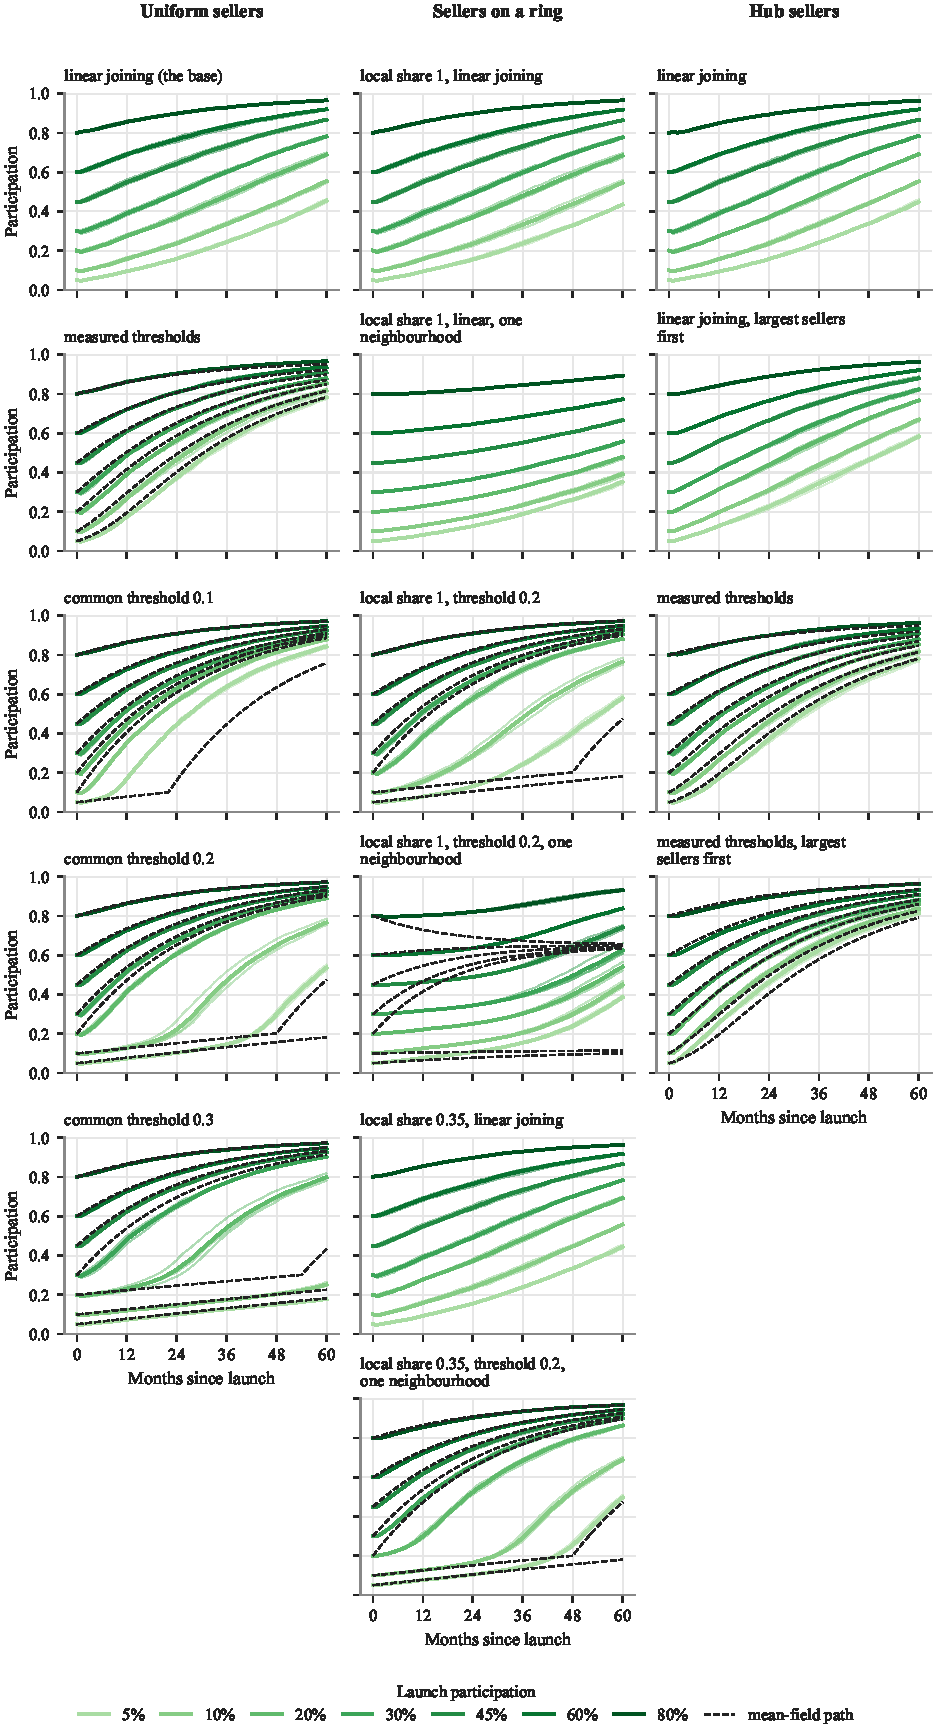
\includegraphics[width=\linewidth,height=0.86\textheight,keepaspectratio]{figures/fig_robust_paths.pdf}
\caption{Participation under CPM month by month in every variant, from the seven launch levels: the seed mean thick
and each seed thin. Dashed lines are the well-mixed path with each person's threshold kept, one leaving rate
fitted.}
\label{fig:robustpaths}
\end{figure}

\begin{figure}[htbp]\centering
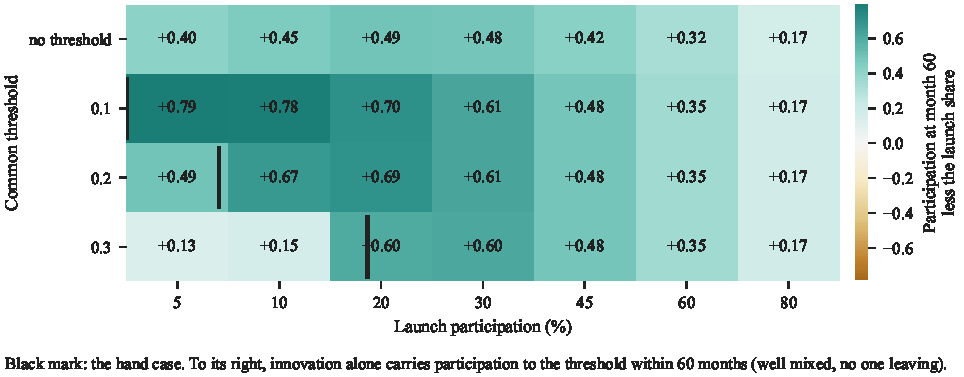
\includegraphics[width=\linewidth]{figures/fig_threshold_map.pdf}
\caption{Participation at month 60 less the launch share, by launch share and common threshold, uniform sellers.
The mark in each row is the hand case: to its right, innovation alone carries a well-mixed population to the
threshold within 60 months.}
\label{fig:thresholdmap}
\end{figure}

\subsection{Chains of failure}\label{sec:chains}

A failed payment is missing income for its payee, so failure can pass from payer to payee. Two readings measure how
far it does.

Within a day each payer's failure is split into the part it would fail even if paid in full that day and the part
due to short receipts, the fundamental and contagious defaults of \cite{elsinger}
(Table~\ref{tab:chains}). The second part is small: \KnockOnBanks{} of failed value under banks and cards and
\KnockOnCpm{} under CPM with no distress, \KnockOnBanksStress{} and \KnockOnCpmStress{} at 2 points. Under CPM it
is lower by \KnockOnGap{} of failed value with no distress (\KnockOnGapRange{} over cells and seeds); at 2 points
the range, \KnockOnGapStressRange{}, includes runs where it is higher. The pool changes who bears it. Under banks
and cards a knock-on failure touches a few payers on most days and never as many as 32. With a pool it touches many
borrowers at once on some days: 32 or more on \ManyKnockOnCpm{} of days under CPM and \ManyKnockOnPool{} in the
pool without the charge, and \ManyKnockOnCpmStress{} and \ManyKnockOnPoolStress{} at 2 points. When receipts fall
short the pool's cash is rationed pro rata, so one payer's shortfall is spread thinly over everyone who borrows that
day. More payers are touched and less value fails.

Across days no such split exists, since a failure today changes every later day. What can be read is how far a
shock spreads. A run at a distress level differs from the same seed's run with no distress only through the extra
layoffs, which can be drawn again from the seed, so the extra failed payments divide between the people an
extra layoff hit and everyone else (Table~\ref{tab:spread}, read on the development map, whose runs store each
person's failed payments). Between \SpreadWideLow{} and \SpreadWideHigh{} of the
excess over the three years from the shock falls on people not laid off, when everything a hit person
fails from its first hit on counts as its own, and \SpreadNarrowLow{} to \SpreadNarrowHigh{} when only what it
fails in a month it is hit does. The shares are alike in every arrangement and mix three channels: income
missing along the payment network, the wages of extra layoffs leaving the household economy, and the shift in
everyone's spending. They measure the spread of distress to people not laid off, not the length of a chain.

In the distress year the excess is lower under CPM than under banks and cards in \SpreadLowerYearHalf{},
\SpreadLowerYearOne{}, \SpreadLowerYearOneHalf{} and \SpreadLowerYearTwo{} of \SpreadCells{} cells at 0.5, 1, 1.5
and 2 points. Over the three years it is lower in \SpreadLowerHalf{}, \SpreadLowerOne{}, \SpreadLowerOneHalf{} and
\SpreadLowerTwo{}. At 2 points the median difference over the three years is \SpreadGapTwo{} failed shares a person
a year, against CPM: where the pool is run, those who relied on it lose more of what they had than those who
never had it. The level of failed payments is still lower under CPM (Table~\ref{tab:arrangements}); the excess is what a
shock adds to each arrangement's own level.

\begin{table}[htbp]\centering\small
\resizebox{\linewidth}{!}{% Written by scripts/paper_numbers.py from confirmation_quote.
\begin{tabular}{llrrrrrrrrrr}
\toprule
Distress & Arrangement & Knock-on share (median) & Knock-on share (range) & Payers a day (median) & Payers a day (range) & Days with 32 or more (median) & Days with 32 or more (range) & Netting share (median) & Netting share (range) & Netting days (median) & Netting days (range) \\
\midrule
None & Banks and cards & 0.57\% & 0.57\% & 2.4 & 2.4 & 0.0\% & 0.0\% & 0.000\% & 0.000\% & 0.0 & 0.0 \\
 & Best-case DeFi & 0.55\% & 0.53\% to 0.56\% & 2.3 & 2.2 to 2.4 & 0.0\% & 0.0\% & 0.000\% & 0.000\% & 0.0 & 0.0 \\
 & Pool without the holding charge & 0.44\% & 0.44\% to 0.52\% & 8.7 & 4.4 to 19.7 & 10.5\% & 4.5\% to 18.8\% & 0.000\% & 0.000\% & 0.0 & 0.0 \\
 & CPM & 0.41\% & 0.41\% to 0.51\% & 5.4 & 3.2 to 10.7 & 5.7\% & 2.6\% to 10.0\% & 0.000\% & 0.000\% & 0.0 & 0.0 \\
 & Indexed CPM & 0.42\% & 0.41\% to 0.51\% & 5.3 & 3.1 to 10.5 & 5.7\% & 2.5\% to 9.9\% & 0.000\% & 0.000\% & 0.0 & 0.0 \\
\midrule
2 points & Banks and cards & 0.84\% & 0.84\% & 3.8 & 3.8 & 0.0\% & 0.0\% & 0.000\% & 0.000\% & 0.0 & 0.0 \\
 & Best-case DeFi & 0.81\% & 0.76\% to 0.82\% & 3.7 & 3.5 to 3.8 & 0.0\% & 0.0\% & 0.000\% & 0.000\% & 0.0 & 0.0 \\
 & Pool without the holding charge & 0.69\% & 0.68\% to 0.78\% & 18.9 & 7.3 to 40.4 & 17.8\% & 7.2\% to 28.7\% & 0.000\% & 0.000\% & 0.0 & 0.0 \\
 & CPM & 0.69\% & 0.65\% to 0.76\% & 15.6 & 5.2 to 34.1 & 13.2\% & 3.7\% to 22.5\% & 0.000\% & 0.000\% & 0.0 & 0.0 \\
 & Indexed CPM & 0.69\% & 0.65\% to 0.79\% & 15.3 & 5.2 to 36.5 & 13.1\% & 3.8\% to 24.3\% & 0.000\% & 0.000\% & 0.0 & 0.0 \\
\bottomrule
\end{tabular}
}
\caption{Failure passed on within a day, on six cells (an outside rate of 4.4\%; launch participation of 5\%, 20\%
and 60\%): the share of failed value that fails only because receipts were short, the payers with such a failure a
day, the share of days when 32 or more payers had one, and the payments that rest on a closed loop of payers
without money. Medians and ranges over the three launch levels of the seed means.}
\label{tab:chains}
\end{table}

\begin{table}[htbp]\centering\small
\resizebox{\linewidth}{!}{% Written by scripts/paper_numbers.py from confirmation_quote.
\begin{tabular}{llrrrrrrr}
\toprule
Distress & Arrangement & Excess (median) & Excess (range) & Not hit, wide & Not hit, narrow & Distress year (median) & Distress year (range) & Not hit, distress year \\
\midrule
0.5 pt & Banks and cards & 0.783 & 0.764 to 0.786 & 0.92 & 0.95 & 0.306 & 0.302 to 0.307 & 0.75 \\
 & Best-case DeFi & 0.754 & 0.702 to 0.774 & 0.92 & 0.94 & 0.305 & 0.296 to 0.314 & 0.73 \\
 & Pool without the holding charge & 0.643 & 0.523 to 1.014 & 0.91 & 0.94 & 0.253 & 0.215 to 0.313 & 0.72 \\
 & CPM & 0.641 & 0.473 to 1.001 & 0.91 & 0.94 & 0.239 & 0.218 to 0.335 & 0.72 \\
\midrule
1 pt & Banks and cards & 1.645 & 1.595 to 1.664 & 0.89 & 0.95 & 0.621 & 0.613 to 0.625 & 0.72 \\
 & Best-case DeFi & 1.579 & 1.459 to 1.613 & 0.89 & 0.95 & 0.626 & 0.614 to 0.655 & 0.70 \\
 & Pool without the holding charge & 1.444 & 1.254 to 2.094 & 0.90 & 0.95 & 0.527 & 0.448 to 0.655 & 0.70 \\
 & CPM & 1.373 & 1.242 to 2.339 & 0.89 & 0.95 & 0.519 & 0.439 to 0.673 & 0.71 \\
\midrule
1.5 pt & Banks and cards & 2.590 & 2.512 to 2.631 & 0.85 & 0.95 & 0.952 & 0.941 to 0.957 & 0.69 \\
 & Best-case DeFi & 2.492 & 2.306 to 2.558 & 0.85 & 0.94 & 0.958 & 0.940 to 0.998 & 0.68 \\
 & Pool without the holding charge & 2.440 & 2.071 to 3.524 & 0.86 & 0.95 & 0.848 & 0.702 to 1.016 & 0.67 \\
 & CPM & 2.286 & 2.075 to 3.735 & 0.86 & 0.94 & 0.841 & 0.647 to 0.997 & 0.67 \\
\midrule
2 pt & Banks and cards & 3.726 & 3.602 to 3.803 & 0.82 & 0.94 & 1.252 & 1.236 to 1.263 & 0.68 \\
 & Best-case DeFi & 3.561 & 3.248 to 3.685 & 0.82 & 0.94 & 1.259 & 1.239 to 1.317 & 0.67 \\
 & Pool without the holding charge & 3.948 & 3.046 to 5.019 & 0.84 & 0.95 & 1.117 & 0.952 to 1.460 & 0.66 \\
 & CPM & 3.919 & 2.999 to 5.223 & 0.84 & 0.95 & 1.084 & 0.861 to 1.413 & 0.66 \\
\bottomrule
\end{tabular}
}
\caption{The extra failed payments at a distress level over the same seed's run with no distress, in failed shares
of bills and wages a person a year, over the three years from the shock and in the distress year: medians and
ranges over the 21 cells of a level of the seed means, with the share that falls on people no extra layoff hit.}
\label{tab:spread}
\end{table}

\subsection{Population size}

Figure~\ref{fig:size} shows the size check beside the choice of \NumPeople{} people (Section~\ref{sec:measurement}): eight seeds kept for nothing
else, at five population sizes. CPM's gains over banks and cards and over best-case DeFi do not move with size.
The gain over the pool without the charge grows with size, so the present population understates what the charge
adds. The count of seeds with a pool run at 2 points rises with size, then levels off: small populations hide
the stress boundary, and it is not an artefact of size.

\begin{figure}[htbp]\centering
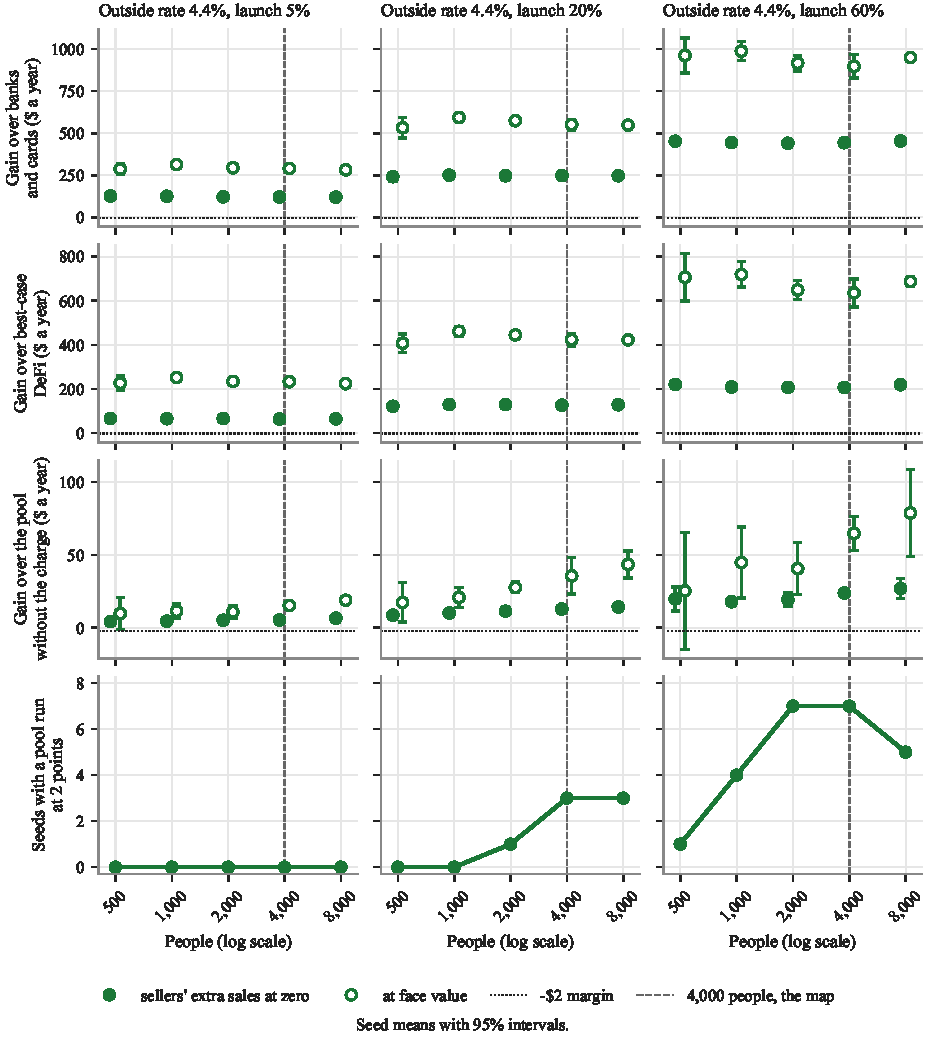
\includegraphics[width=0.92\linewidth]{figures/fig_size_check.pdf}
\caption{The population size check, three cells at an outside rate of 4.4\%: CPM's gain over banks and cards, over
best-case DeFi and over the pool without the charge, and the number of seeds, of eight, with a pool run at 2
points of distress, against population size.}
\label{fig:size}
\end{figure}
